% Progress Update Presentation
% Cloud Native Analytical Database Benchmarking
% Farbod Mohammadzadeh

\documentclass[aspectratio=169]{beamer}

% ============================================
% THEME AND COLORS
% ============================================
\usetheme{Madrid}
\usecolortheme{default}

% Custom colors
\definecolor{uoftblue}{RGB}{0, 42, 92}
\definecolor{accentblue}{RGB}{30, 100, 200}

\setbeamercolor{structure}{fg=uoftblue}
\setbeamercolor{title}{fg=white,bg=uoftblue}
\setbeamercolor{frametitle}{fg=white,bg=uoftblue}
\setbeamercolor{block title}{fg=white,bg=accentblue}

% ============================================
% PACKAGES
% ============================================
\usepackage{graphicx}
\usepackage{booktabs}
\usepackage{tikz}
\usetikzlibrary{shapes,arrows,positioning}
\usepackage{pgfgantt}

% Remove navigation symbols
\setbeamertemplate{navigation symbols}{}

% Add frame numbers
\setbeamertemplate{footline}[frame number]

% ============================================
% TITLE PAGE INFO
% ============================================
\title[Cloud DB Benchmarking]{Cloud Native Analytical Database Benchmarking}
\subtitle{Progress Update}
\author{Farbod Mohammadzadeh}
% \institute{Supervisor: Professor Arno Jacobsen\\University of Toronto}
\date{January 2026}

% ============================================
% DOCUMENT
% ============================================
\begin{document}

% --------------------------------------------
% TITLE SLIDE
% --------------------------------------------
\begin{frame}
    \titlepage
\end{frame}

% --------------------------------------------
% OUTLINE
% --------------------------------------------
\begin{frame}{Outline}
    \tableofcontents
\end{frame}

% ============================================
% SECTION 1: INTRODUCTION & MOTIVATION
% ============================================
\section{Introduction \& Motivation}

\begin{frame}{Recap: Research Gap \& Objectives}
    \textbf{The Problem:} TPC benchmarks don't reflect real cloud workloads
    \begin{itemize}
        \item Production: 50\%+ writes, heavy-tailed latencies, dynamic concurrency
        \item Prior work addresses hardware OR structure---not both
    \end{itemize}
    
    \vspace{0.4cm}
    \textbf{This Thesis:} Unified benchmark matching \emph{both} dimensions
    
    \vspace{0.3cm}
    \begin{columns}
        \column{0.33\textwidth}
        \centering
        \textbf{Objective 1}\\[0.2cm]
        Workload synthesis pipeline
        
        \column{0.33\textwidth}
        \centering
        \textbf{Objective 2}\\[0.2cm]
        Cross-config benchmark dataset
        
        \column{0.33\textwidth}
        \centering
        \textbf{Objective 3}\\[0.2cm]
        Rigorous validation
    \end{columns}
\end{frame}

% ============================================
% SECTION 2: METHODOLOGY
% ============================================
\section{Methodology}

\begin{frame}{Overall Approach}
    \begin{center}
        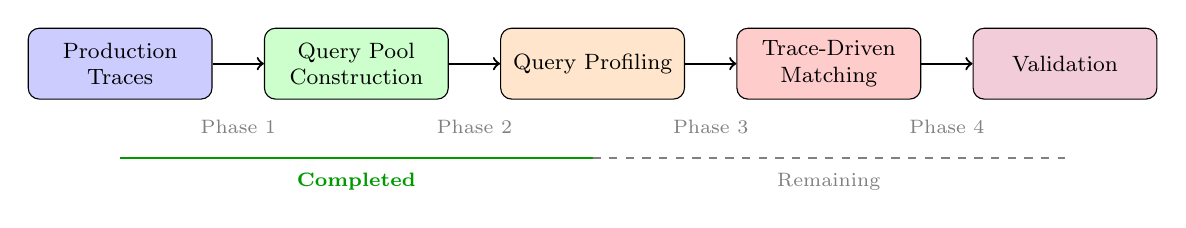
\begin{tikzpicture}[
            box/.style={rectangle, draw, rounded corners, minimum width=2.3cm, minimum height=0.9cm, text width=2.1cm, align=center, font=\footnotesize},
            arrow/.style={->, thick}
        ]
            \node[box, fill=blue!20] (trace) at (0,0) {Production Traces};
            \node[box, fill=green!20] (pool) at (3,0) {Query Pool Construction};
            \node[box, fill=orange!20] (profile) at (6,0) {Query Profiling};
            \node[box, fill=red!20] (match) at (9,0) {Trace-Driven Matching};
            \node[box, fill=purple!20] (valid) at (12,0) {Validation};
            
            \draw[arrow] (trace) -- (pool);
            \draw[arrow] (pool) -- (profile);
            \draw[arrow] (profile) -- (match);
            \draw[arrow] (match) -- (valid);
            
            % Phase labels
            \node[font=\scriptsize, gray] at (1.5,-0.8) {Phase 1};
            \node[font=\scriptsize, gray] at (4.5,-0.8) {Phase 2};
            \node[font=\scriptsize, gray] at (7.5,-0.8) {Phase 3};
            \node[font=\scriptsize, gray] at (10.5,-0.8) {Phase 4};
            
            % Current progress indicator
            \draw[thick, green!60!black] (0,-1.2) -- (6,-1.2);
            \draw[thick, gray, dashed] (6,-1.2) -- (12,-1.2);
            \node[font=\scriptsize, green!60!black] at (3,-1.5) {\textbf{Completed}};
            \node[font=\scriptsize, gray] at (9,-1.5) {Remaining};
        \end{tikzpicture}
    \end{center}
    
    \vspace{0.3cm}
    \textbf{Key components:}
    \begin{itemize}
        \item Multi-objective optimization 
        \item LLM-based query augmentation 
        \item Learned performance prediction
    \end{itemize}
\end{frame}

% ============================================
% SECTION 3: WORK COMPLETED
% ============================================
\section{Work Completed}

\begin{frame}{Infrastructure Setup}
    \textbf{Analysis Infrastructure:}
    \begin{itemize}
        \item DuckDB-based views architecture for production traces
        \item Memory-efficient querying of 500M+ records
        \item Parameterized sampling for iterative analysis
    \end{itemize}
    
    \vspace{0.4cm}
    \textbf{Benchmark Infrastructure:}
    \begin{itemize}
        \item TPC-DS Scale Factor 1 (1 GB, 24 tables) + TPC-H Scale Factor 1 (8 tables)
        \item Official DSGen 4.0.0 and DBGen data generation
        \item Persistent DuckDB storage for reproducible profiling
    \end{itemize}
    
    \vspace{0.4cm}
    \textbf{Profiling Environment:}
    \begin{itemize}
        \item Lightweight Alpine Linux VMs with configurable resources
        \item Currently varying: vCPUs (2--8), RAM (2--8 GB)
        \item Metric focus: execution time (hardware counters planned)
    \end{itemize}
\end{frame}

\begin{frame}{Datasets Analyzed}
    \begin{table}
        \centering
        \begin{tabular}{lccc}
            \toprule
            \textbf{Dataset} & \textbf{Queries} & \textbf{Columns} & \textbf{Key Features} \\
            \midrule
            Snowset & 69.2M & 93 & Operator-level CPU breakdown \\
            Redset Serverless & 8.2M & 24 & Query type, cache hits \\
            Redset Provisioned & 433.1M & 24 & Large scale validation \\
            \bottomrule
        \end{tabular}
    \end{table}
    
    \vspace{0.3cm}
    \textbf{All datasets:}
    \begin{itemize}
        \item Stored in Parquet format with time-series partitioning
        \item Unified analysis via DuckDB views
        \item No data duplication overhead
    \end{itemize}
\end{frame}

\begin{frame}{Key Findings from Trace Analysis (Recap)}
    \textbf{Previously presented findings that drive the synthesis approach:}
    
    \vspace{0.3cm}
    \begin{columns}
        \column{0.5\textwidth}
        \textbf{Workload Characteristics:}
        \begin{itemize}
            \item Heavy-tailed durations (P95/median: 100$\times$+)
            \item 50\%+ write operations (vs. TPC's 100\% SELECT)
            \item Scan-dominated CPU (40\%), I/O-bound
        \end{itemize}
        
        \column{0.5\textwidth}
        \textbf{Novel Discoveries:}
        \begin{itemize}
            \item Saturation threshold at $\sim$110 concurrent queries
            \item Non-monotonic warehouse scaling (self-selection)
            \item Low cache hits despite high repetition
        \end{itemize}
    \end{columns}
    
    \vspace{0.4cm}
    \begin{block}{Implication for Synthesis}
        These characteristics define our matching targets---the synthetic workload must reproduce these patterns.
    \end{block}
\end{frame}

\begin{frame}{TPC-DS \& TPC-H Baseline Profiling}
    \textbf{Completed:}
    \begin{itemize}
        \item 99 TPC-DS + 22 TPC-H query templates profiled
        \item Executed in Alpine Linux VMs with varying CPU/RAM configs
        \item Current metric: execution time; hardware counters planned
    \end{itemize}
    
    \vspace{0.3cm}
    \textbf{Confirmed gaps vs. production:}
    \begin{itemize}
        \item Tighter execution time clustering (uniform data)
        \item Only SELECT queries (no writes, no metadata)
        \item Inner-join bias (production: 37\% outer joins)
        \item Numeric keys (production: 50\% text-based keys)
    \end{itemize}
    
    \vspace{0.3cm}
    \begin{alertblock}{Implication}
        Query pool requires substantial augmentation before it can approximate real workloads.
    \end{alertblock}
\end{frame}

\begin{frame}{LLM Augmentation: Preliminary Work}
    \textbf{Initial experiments completed:}
    \begin{itemize}
        \item Using TPC-H/DS queries as seed inputs for LLM-based generation
        \item Testing structural modifications: adding outer joins, text predicates, CTEs
    \end{itemize}
    
    \vspace{0.3cm}
    \textbf{OpenAI models evaluated:}
    \begin{itemize}
        \item GPT-4o-mini: Fast, cost-effective for bulk generation
        \item GPT-4o: Higher quality but slower; better for complex transformations
        \item Quick observation: smaller models struggle with schema consistency
    \end{itemize}
    
    \vspace{0.3cm}
    \textbf{Under consideration: Cross-AI Validation}
    \begin{itemize}
        \item Use one model to generate, another to validate/critique
        \item Potential for catching hallucinations and schema errors
        \item Exploring Claude, Gemini as validation backends
    \end{itemize}
\end{frame}

% ============================================
% SECTION 4: FUTURE WORK
% ============================================
\section{Future Work}

\begin{frame}{Remaining Work: Phase 3 -- LLM Augmentation}
    \textbf{Two complementary LLM strategies under consideration:}
    
    \vspace{0.2cm}
    \begin{columns}
        \column{0.5\textwidth}
        \textbf{SQLBarber-style (Controlled):}
        \begin{itemize}
            \item User-specified structural constraints
            \item LLM generates SQL \emph{templates}
            \item Self-correction loop for validation
            \item Bayesian optimization for instantiation
        \end{itemize}
        
        \column{0.5\textwidth}
        \textbf{SQLStorm-style (Diverse):}
        \begin{itemize}
            \item Large-scale stochastic generation
            \item Generate-and-filter pipeline
            \item LLM rewriting for compatibility
            \item Maximizes query plan diversity
        \end{itemize}
    \end{columns}
    
    \vspace{0.3cm}
    \textbf{Targets:} Write operations, metadata queries, outer joins, text keys, CTEs
    
    \vspace{0.2cm}
    \textbf{Multi-Environment Profiling (expanding current Alpine VM setup):}
    \begin{itemize}
        \item Scale to 2--16 vCPUs, 4--32 GB RAM, SF 1--100
        \item Add hardware dimensions: CPU cycles, cache misses, I/O wait
    \end{itemize}
\end{frame}

\begin{frame}{Remaining Work: Matching Algorithm}
    \textbf{Three-stage approach:}
    
    \vspace{0.2cm}
    \begin{enumerate}
        \item \textbf{Database Assignment \& Filtering}
        \begin{itemize}
            \item Map trace databases to test databases
            \item Filter compatible queries
        \end{itemize}
        
        \vspace{0.2cm}
        \item \textbf{Performance Matching}
        \begin{itemize}
            \item Match CPU time and duration targets
            \item Account for concurrency effects
        \end{itemize}
        
        \vspace{0.2cm}
        \item \textbf{Structural Balance}
        \begin{itemize}
            \item Verify aggregate operator distributions
            \item Bias assignments toward underrepresented categories
        \end{itemize}
    \end{enumerate}
    
    \vspace{0.3cm}
    \textbf{Optimization approaches to explore:} ILP, simulated annealing, LLM-guided search
\end{frame}

\begin{frame}{Remaining Work: Phase 4 Validation}
    \textbf{Four validation dimensions:}
    
    \begin{enumerate}
        \item \textbf{Performance Fidelity}
        \begin{itemize}
            \item CPU time distribution, duration percentiles, throughput
        \end{itemize}
        
        \item \textbf{Structural Fidelity}
        \begin{itemize}
            \item Operator distributions, join patterns, complexity
        \end{itemize}
        
        \item \textbf{Temporal Dynamics}
        \begin{itemize}
            \item Concurrency patterns, peak loads, saturation behavior
        \end{itemize}
        
        \item \textbf{Cross-Deployment Generalization}
        \begin{itemize}
            \item Verify workloads behave consistently across hardware configs
            \item Relative performance relationships should hold
        \end{itemize}
    \end{enumerate}
\end{frame}

\begin{frame}{Success Metrics}
    \begin{table}
        \centering
        \begin{tabular}{lc}
            \toprule
            \textbf{Metric} & \textbf{Target} \\
            \midrule
            KL divergence (duration distributions) & $< 0.1$ \\
            Operator type proportions & $\pm 10\%$ of target \\
            Peak/median concurrency & $\pm 15\%$ of trace \\
            Cross-deployment stability & 3+ configurations \\
            \bottomrule
        \end{tabular}
    \end{table}
    
    \vspace{0.3cm}
    \textbf{Deliverables:}
    \begin{itemize}
        \item Workload synthesis pipeline (open-source)
        \item Augmented query pool (TPC-DS + TPC-H + writes + metadata)
        \item Performance profile database
        \item Validation dataset with comparative metrics
    \end{itemize}
\end{frame}

\begin{frame}[fragile]{Timeline}
    \begin{center}
        \begin{ganttchart}[
            hgrid,
            vgrid,
            x unit=0.9cm,
            y unit chart=0.5cm,
            title height=1,
            bar/.style={fill=blue!50},
            bar height=0.5,
            group/.style={fill=blue!80},
            milestone/.style={fill=red!70}
        ]{1}{8}
            \gantttitle{2025}{4}
            \gantttitle{2026}{4} \\
            \gantttitle{Sep}{1}
            \gantttitle{Oct}{1}
            \gantttitle{Nov}{1}
            \gantttitle{Dec}{1} 
            \gantttitle{Jan}{1}
            \gantttitle{Feb}{1}
            \gantttitle{Mar}{1}
            \gantttitle{Apr}{1} \\
            
            \ganttbar[bar/.style={fill=green!50}]{Trace Analysis}{1}{2} \\
            \ganttbar[bar/.style={fill=green!50}]{TPC-DS Setup}{2}{3} \\
            \ganttbar[bar/.style={fill=green!50}]{Query Profiling}{3}{4} \\
            \ganttbar[bar/.style={fill=yellow!50}]{LLM Augmentation}{4}{5} \\
            \ganttbar{Multi-VM Profiling}{5}{5} \\
            \ganttbar{Matching Algorithm}{5}{6} \\
            \ganttbar{Validation}{6}{7} \\
            \ganttbar{Thesis Writing}{7}{7} \\
            \ganttmilestone{Submission}{7.8}
        \end{ganttchart}
    \end{center}
    
    \textcolor{green!60!black}{$\blacksquare$ Completed} \quad
    \textcolor{yellow!70!black}{$\blacksquare$ In Progress} \quad
    \textcolor{blue!50}{$\blacksquare$ Planned}
\end{frame}

\begin{frame}{Risk Mitigation}
    \begin{columns}
        \column{0.5\textwidth}
        \textbf{Technical Risks:}
        \begin{itemize}
            \item LLM query quality $\rightarrow$ validation pipeline with self-correction
            \item Performance prediction accuracy $\rightarrow$ fallback to learned models
            \item Matching convergence $\rightarrow$ incremental constraint relaxation
        \end{itemize}
        
        \column{0.5\textwidth}
        \textbf{Resource Risks:}
        \begin{itemize}
            \item Compute costs $\rightarrow$ spot instances, subset profiling first
            \item LLM API costs $\rightarrow$ smaller models for bulk work
            \item Schedule delays $\rightarrow$ early validation, documented scripts
        \end{itemize}
    \end{columns}
    
    \vspace{0.5cm}
    \textbf{Alternative approaches ready:}
    \begin{itemize}
        \item Fully generative synthesis (SQLStorm-style) if component-based insufficient
        \item Learned performance prediction (Stitcher-style) if analytical models fail
    \end{itemize}
\end{frame}

% ============================================
% SUMMARY
% ============================================
\section{Summary}

\begin{frame}{Summary}
    \textbf{Progress:}
    \begin{itemize}
        \item Analyzed 500M+ production queries across Snowset and Redset
        \item Quantified gaps between TPC benchmarks and real workloads
        \item Established benchmark infrastructure (TPC-DS + TPC-H, profiling framework)
        % \item Discovered novel insights (saturation threshold, scaling variance)
    \end{itemize}
    
    \vspace{0.3cm}
    \textbf{Next Steps:}
    \begin{itemize}
        \item Complete query pool augmentation with LLM-generated queries
        \item Implement trace-driven matching algorithm
        \item Validate across multiple deployment configurations
    \end{itemize}
    
    \vspace{0.3cm}
    \textbf{Goal:} A benchmark generator that produces tests reflecting actual customer usage.
\end{frame}

\begin{frame}
    \centering
    \Huge{\textbf{Questions?}}
\end{frame}

\end{document}
